%%%%%%%%%%%%%%%%%%%%%%%%%%%%%%%%%%%%
% Slide options
%%%%%%%%%%%%%%%%%%%%%%%%%%%%%%%%%%%%

% Option 1: Slides with solutions

\documentclass[slidestop,compress,mathserif]{beamer}
\usepackage{booktabs}
\newcommand{\soln}[1]{\textit{#1}}
\newcommand{\solnGr}[1]{#1}

% Option 2: Handouts without solutions

%\documentclass[11pt,containsverbatim,handout]{beamer}
%\usepackage{pgfpages}
%\pgfpagesuselayout{4 on 1}[letterpaper,landscape,border shrink=5mm]
%\newcommand{\soln}[1]{ }
%\newcommand{\solnGr}{ }

%%%%%%%%%%%%%%%%%%%%%%%%%%%%%%%%%%%%
% Style
%%%%%%%%%%%%%%%%%%%%%%%%%%%%%%%%%%%%
%%%%%%%%%%%%%%%%%%%%%%%%%%%%%%%%%%%%%%%%%%%%%%%%%%%%%%%%%%%%%%%%%%%%%%%%
% MA213/214 shared slide style
%
% "Calm & Cool" palette + content-type callout boxes.
% Overhauled (2026) from the original OpenIntro/metropolis style:
%   - all OpenIntro visual branding removed (logo, grid, colors)
%   - a low-key cool palette (see colors below)
%   - tcolorbox callout boxes so students recognize content types
% See common/README.md for the command cheat-sheet.
%%%%%%%%%%%%%%%%%%%%%%%%%%%%%%%%%%%%%%%%%%%%%%%%%%%%%%%%%%%%%%%%%%%%%%%%

\usetheme{metropolis}

%%%%%%%%%%%%%%%%
% Packages
%%%%%%%%%%%%%%%%

\usepackage{geometry}
\usepackage{graphicx}
\usepackage{amssymb}
\usepackage{epstopdf}
\usepackage{amsmath}  	% this permits text in eqnarray among other benefits
\usepackage{url}		% produces hyperlinks
\usepackage{hyperref}	% allows for color usage in tables
\usepackage[english]{babel}
\usepackage[latin1]{inputenc}
\usepackage{colortbl}	% allows for color usage in tables
\usepackage{multirow}	% allows for rows that span multiple rows in tables
\usepackage{color}		% this package has a variety of color options
\usepackage{pgf}
\usepackage{calc}
\usepackage{ulem}
\usepackage{multicol}
\usepackage{textcomp}
\usepackage{txfonts}
\usepackage{listings}
\usepackage{tikz}
\usepackage{array}
\usepackage{wasysym}
\usepackage{fancyvrb}
\usepackage{etoolbox}             % \ifstrempty for optional box subtitles
\usepackage[most]{tcolorbox}      % content-type callout boxes
\tcbuselibrary{listings}          % R-code block (\begin{rblock})
\usepackage{fontawesome5}         % box icons

%%%%%%%%%%%%%%%%
% Remove navigation symbols
%%%%%%%%%%%%%%%%

\setbeamertemplate{navigation symbols}{}

%%%%%%%%%%%%%%%%
% "Calm & Cool" palette
%%%%%%%%%%%%%%%%

% chrome / structure / body
\definecolor{ccSlate}{HTML}{2E3742}   % frametitle bar, structure, section pages (deep neutral slate)
\definecolor{ccInk}{HTML}{2B2B2B}     % body text
\definecolor{ccWash}{HTML}{FCF8F1}    % gentle warm title-slide background wash (complements the cool blues)

% example (blue)
\definecolor{ccBlue}{HTML}{2F6690}
\definecolor{ccBlueBg}{HTML}{EAF1F7}
% interactive activity / discussion (green)
\definecolor{ccGreen}{HTML}{4E8A6B}
\definecolor{ccGreenBg}{HTML}{E9F3EC}
% solution (purple)
\definecolor{ccPurple}{HTML}{6F5499}
\definecolor{ccPurpleBg}{HTML}{EFEAF6}
% worksheet / focused work (terracotta)
\definecolor{ccTerra}{HTML}{C2693E}
\definecolor{ccTerraBg}{HTML}{FAEDE4}
% formula / definition (neutral slate)
\definecolor{ccGray}{HTML}{5C6B7A}
\definecolor{ccGrayBg}{HTML}{EEF1F4}
% caution / common pitfall (brick red)
\definecolor{ccRed}{HTML}{B23A48}
\definecolor{ccRedBg}{HTML}{FAEAEC}
% key idea / takeaway (muted gold)
\definecolor{ccGold}{HTML}{9C7A28}
\definecolor{ccGoldBg}{HTML}{F7F1DF}
% learning goals / lesson outcomes (teal)
\definecolor{ccTeal}{HTML}{2C6E6B}
\definecolor{ccTealBg}{HTML}{E6F0EF}
% learning objectives (indigo)
\definecolor{ccIndigo}{HTML}{45507A}
\definecolor{ccIndigoBg}{HTML}{ECEEF4}
% R code / output (gray)
\definecolor{ccCode}{HTML}{5F5E5A}
\definecolor{ccCodeBg}{HTML}{F4F5F6}

% neutral grays kept from the original style
\definecolor{gray}{rgb}{0.5, 0.5, 0.5}
\definecolor{darkGray}{rgb}{0.3, 0.3, 0.3}
\definecolor{darkerGray}{rgb}{0.2, 0.2, 0.2}

% Backwards-compatible aliases: old OpenIntro color names now point at the
% new palette, so existing \textcolor{oiB}{...}, \hl{...}, etc. keep working.
\colorlet{oiB}{ccBlue}
\colorlet{oiG}{ccGreen}
\colorlet{hlblue}{ccBlue}
\colorlet{rubineRed}{ccRed}
\colorlet{irishGreen}{ccGreen}
\colorlet{lightGreen}{ccGreen}

%%%%%%%%%%%%%%%%
% Restyle metropolis with the Calm & Cool chrome
%%%%%%%%%%%%%%%%

\metroset{block=fill}

\setbeamercolor{normal text}{fg=ccInk, bg=white}
\setbeamercolor{structure}{fg=ccSlate}
\setbeamercolor{alerted text}{fg=ccBlue}
\setbeamercolor{example text}{fg=ccGreen}
\setbeamercolor{frametitle}{bg=ccSlate, fg=white}
\setbeamercolor{progress bar}{fg=ccBlue}
\setbeamercolor{title separator}{fg=ccBlue}
\setbeamercolor{title}{fg=ccSlate}
\setbeamercolor{subtitle}{fg=ccBlue}
\setbeamercolor{author}{fg=ccInk}
\setbeamercolor{institute}{fg=ccGray}
\setbeamercolor{date}{fg=ccGray}
\setbeamercolor{section title}{fg=ccSlate}
\setbeamercolor{standout}{fg=white, bg=ccSlate}

% Section pages sit on the same warm wash as the title slide. We keep
% metropolis's section-title styling and just paint a full-page ccWash
% background behind it (needs >=2 pdflatex passes for the current-page node).
\setbeamertemplate{section page}{%
  \begin{tikzpicture}[remember picture, overlay]
    \fill[ccWash] (current page.south west) rectangle (current page.north east);
  \end{tikzpicture}%
  \centering
  \begin{minipage}{22em}
    \raggedright
    \usebeamercolor[fg]{section title}%
    \usebeamerfont{section title}%
    \insertsectionhead\\[-1ex]
    \usebeamertemplate*{progress bar in section page}%
    \par
  \end{minipage}\par
  \vspace{\baselineskip}
}

%%%%%%%%%%%%%%%%
% Custom inline text commands (recolored to the palette)
%%%%%%%%%%%%%%%%

% degree
\newcommand{\degree}{\ensuremath{^\circ}}

% cite
\newcommand{\ct}[1]{
\vfill
{\tiny #1}}

\newcommand{\NamedNote}[2]{
\rule{2.5cm}{0.25pt} \\ \textit{\footnotesize{\textcolor{rubineRed}{#1:} \textcolor{darkerGray}{#2}}}}

% Note
\newcommand{\Note}[1]{
\rule{2.5cm}{0.25pt} \\ \textit{\footnotesize{\textcolor{rubineRed}{Note:} \textcolor{darkerGray}{#1}}}}

% Remember
\newcommand{\Remember}[1]{\textit{\scriptsize{\textcolor{ccTerra}{Remember:} #1}}}

% expected counts
\newcommand{\ex}[1]{\textit{\textcolor{ccBlue}{#1}}}

% red
\newcommand{\red}[1]{\textit{\textcolor{rubineRed}{#1}}}

% pink
\newcommand{\pink}[1]{\textit{\textcolor{rubineRed!90!white!50}{#1}}}

% green
\newcommand{\green}[1]{\textit{\textcolor{irishGreen}{#1}}}

% orange
\newcommand{\orange}[1]{\textit{\textcolor{ccTerra}{#1}}}

% links: webURL, webLink, appLink
\newcommand{\webURL}[1]{\urlstyle{same}{ \textit{\textcolor{darkGray}{\url{#1}}}}}
\newcommand{\webLink}[2]{\href{#1}{\textcolor{darkGray}{{#2}}}}
\newcommand{\appLink}[2]{\href{#1}{\textcolor{white}{{#2}}}}

% mail
\newcommand{\mail}[1]{\href{mailto:#1}{\textit{\textcolor{darkGray}{#1}}}}

% highlighting: hl, hlGr, mathhl
\newcommand{\hl}[1]{\textit{\textcolor{hlblue}{#1}}}
\newcommand{\hlGr}[1]{\textit{\textcolor{lightGreen}{#1}}}
\newcommand{\mathhl}[1]{\textcolor{hlblue}{\ensuremath{#1}}}

%%%%%%%%%%%%%%%%
% Structural helpers (unchanged from the original)
%%%%%%%%%%%%%%%%

% two col: two columns
\newenvironment{twocol}[4]{
\begin{columns}[c]
\column{#1\textwidth}
#3
\column{#2\textwidth}
#4
\end{columns}
}

% slot (for probability calculations)
\newenvironment{slot}[2]{
\begin{array}{c}
\underline{#1} \\
#2
\end{array}
}

% pr: left and right parentheses
\newcommand{\pr}[1]{
\left( #1 \right)
}

% cancel
\newcommand{\cancel}[1]{%
    \tikz[baseline=(tocancel.base)]{
        \node[inner sep=0pt,outer sep=0pt] (tocancel) {#1};
        \draw[red, line width=0.5mm] (tocancel.south west) -- (tocancel.north east);
    }%
}

% removepagenumbers
\newcommand{\removepagenumbers}{%
  \setbeamertemplate{footline}{}
}

% change margin
\newenvironment{changemargin}[2]{%
\begin{list}{}{%
\setlength{\topsep}{0pt}%
\setlength{\leftmargin}{#1}%
\setlength{\rightmargin}{#2}%
\setlength{\listparindent}{\parindent}%
\setlength{\itemindent}{\parindent}%
\setlength{\parsep}{\parskip}%
}%
\item}{\end{list}}

% footnote
\long\def\symbolfootnote[#1]#2{\begingroup%
\def\thefootnote{\fnsymbol{footnote}}\footnote[#1]{#2}\endgroup}

% commands from the book
\newenvironment{data}[1]{\texttt{#1}}{}
\newenvironment{var}[1]{\texttt{#1}}{}
\newenvironment{resp}[1]{\texttt{#1}}{}

%%%%%%%%%%%%%%%%
% Content-type callout boxes (tcolorbox)
%
% Each type has a colored title strip (icon + label) over a light fill.
% Color = content type; the label + icon reinforce it (so the cue does
% not rely on color alone).
%%%%%%%%%%%%%%%%

\tcbset{
  cccallout/.style 2 args={
    enhanced, breakable=false,
    colback=#2, colframe=#1, colbacktitle=#1, coltitle=white,
    fonttitle=\bfseries\footnotesize,
    boxrule=0.6pt, arc=2.5pt, outer arc=2.5pt,
    left=5pt, right=5pt, top=3pt, bottom=3pt, boxsep=2pt,
    toptitle=2pt, bottomtitle=2pt, lefttitle=5pt,
    before skip=5pt, after skip=5pt,
  },
}

% One-off / collection of examples (blue): \workedexample[subtitle]{body}.
% (Named \workedexample, not \example, because beamer defines \example.)
\newtcolorbox{examplebox}[1][]{cccallout={ccBlue}{ccBlueBg},
  title={\faIcon{lightbulb}~~Example\ifstrempty{#1}{}{ \textmd{---}\ #1}}}
\newcommand{\workedexample}[2][]{\begin{examplebox}[#1]#2\end{examplebox}}

% Running-example header (blue): \examplehead{name} at the top of each frame of a
% multi-slide running example. A one-off or a collection of examples uses the
% \workedexample box above instead.
\newcommand{\examplehead}[1]{%
  \vspace{-0.4em}\par\noindent\tcbox[on line, colback=ccBlue, colframe=ccBlue, coltext=white,
    boxrule=0pt, arc=2pt, left=5pt, right=5pt, top=1pt, bottom=1pt,
    box align=base, nobeforeafter]{\footnotesize\bfseries\faIcon{lightbulb}\,Running example}%
  \ifstrempty{#1}{}{\enspace{\footnotesize\bfseries\textcolor{ccBlue}{#1}}}%
  \par\nobreak\vspace{-0.6em}{\color{ccBlue}\rule{\linewidth}{0.7pt}}\par\nobreak\vspace{-0.8em}}

% Interactive activity (green): \activity[subtitle]{body}
\newtcolorbox{activitybox}[1][]{cccallout={ccGreen}{ccGreenBg},
  title={\faIcon{users}~~Activity\ifstrempty{#1}{}{ #1}}}
\newcommand{\activity}[2][]{\begin{activitybox}[#1]#2\end{activitybox}}

% Discussion question (green): \dq{body}
\newtcolorbox{dqbox}{cccallout={ccGreen}{ccGreenBg}, title={\faIcon{comments}~~Discussion}}
\newcommand{\dq}[1]{\begin{dqbox}#1\end{dqbox}}

% Solution (purple): \solnbox{body}. Gated by the per-deck \soln toggle, so it
% shows in the instructor build and vanishes from the student handout build.
% (Named \solnbox, not \solution, because beamer already defines \solution.)
\newtcolorbox{solutionbox}{cccallout={ccPurple}{ccPurpleBg}, title={\faIcon{key}~~Solution}}
\newcommand{\solnbox}[1]{\soln{\begin{solutionbox}#1\end{solutionbox}}}

% Worksheet / focused work (terracotta): \worksheet[subtitle]{body}
\newtcolorbox{worksheetbox}[1][]{cccallout={ccTerra}{ccTerraBg},
  title={\faIcon{pencil-alt}~~Worksheet\ifstrempty{#1}{}{ #1}}}
\newcommand{\worksheet}[2][]{\begin{worksheetbox}[#1]#2\end{worksheetbox}}

% Formula / definition (neutral slate). Supports both real usages found in the
% decks: \formula{title}{body} and the bare \formula{body} (title defaults to
% "Formula"). The second group is an optional brace argument.
\newtcolorbox{formulabox}[1][Formula]{cccallout={ccGray}{ccGrayBg},
  title={\faIcon{square-root-alt}~~#1}}
\NewDocumentCommand{\formula}{m g}{%
  \IfNoValueTF{#2}%
    {\begin{formulabox}#1\end{formulabox}}%
    {\begin{formulabox}[#1]#2\end{formulabox}}}

% Common pitfall / caution (brick red): \caution[subtitle]{body}
\newtcolorbox{cautionbox}[1][]{cccallout={ccRed}{ccRedBg},
  title={\faIcon{exclamation-triangle}~~Caution\ifstrempty{#1}{}{ #1}}}
\newcommand{\caution}[2][]{\begin{cautionbox}[#1]#2\end{cautionbox}}

% Key idea / takeaway (muted gold): \keyidea[subtitle]{body}
\newtcolorbox{keyideabox}[1][]{cccallout={ccGold}{ccGoldBg},
  title={\faIcon{star}~~Key idea\ifstrempty{#1}{}{ #1}}}
\newcommand{\keyidea}[2][]{\begin{keyideabox}[#1]#2\end{keyideabox}}

% Learning goals / lesson outcomes (teal): \goals{body}. Sits under the short
% LO headings on the objectives slide; body is the "you should be able to" list.
\newtcolorbox{goalsbox}{cccallout={ccTeal}{ccTealBg}, fontupper=\footnotesize,
  top=1pt, bottom=2pt, boxsep=1pt, before skip=3pt,
  title={\faIcon{bullseye}~~By the end of today, you should be able to\ldots}}
\newcommand{\goals}[1]{\begin{goalsbox}#1\end{goalsbox}}

% Learning objectives (indigo): \objectives{body} -- the formal LO headings,
% shown alongside \goals on the objectives slide.
\newtcolorbox{objectivesbox}{cccallout={ccIndigo}{ccIndigoBg}, fontupper=\small,
  top=1pt, bottom=2pt, boxsep=1pt, before skip=3pt,
  title={\faIcon{clipboard-list}~~Learning objectives}}
\newcommand{\objectives}[1]{\begin{objectivesbox}#1\end{objectivesbox}}

% Defaults for a bare \begin{lstlisting}. Without these it inherits the listings
% package defaults: 11pt type, fixed-width columns (which spaces code out as
% "a g e _ f i t"), and no line breaking, so a long line silently runs off the
% right edge of the slide. A deck that passes its own basicstyle still wins.
% Layout only -- syntax coloring is left to the \begin{rblock} environment.
\lstset{
  basicstyle=\ttfamily\footnotesize, columns=fullflexible,
  breaklines=true, breakindent=1.5em, showstringspaces=false,
  numbers=none, frame=none}

% R code / output (gray): \begin{rblock}[subtitle] ... \end{rblock}
% NOTE: a frame containing an rblock must be declared \begin{frame}[fragile].
\lstdefinestyle{ccR}{
  language=R, basicstyle=\ttfamily\footnotesize, columns=fullflexible,
  breaklines=true, showstringspaces=false, numbers=none, frame=none,
  keywordstyle=\color{ccBlue}, commentstyle=\color{ccGreen!75!black},
  stringstyle=\color{ccTerra}}
\newtcblisting{rblock}[1][]{cccallout={ccCode}{ccCodeBg},
  title={\faIcon{terminal}~~R\ifstrempty{#1}{}{ #1}},
  listing only, listing style=ccR}

% --- Legacy boxes (kept so existing decks compile) ---

% app: application exercise -> alias of activity
\newcommand{\app}[1]{\activity{#1}}

% pq: practice question (green, interactive family)
\newtcolorbox{pqbox}{cccallout={ccGreen}{ccGreenBg}, title={\faIcon{list-ol}~~Practice}}
\newcommand{\pq}[1]{\begin{pqbox}#1\end{pqbox}}

% solnMult: solutions for multiple-choice practice questions (uses \soln toggle)
\newcommand{\solnMult}[1]{
\item[] \vspace{-0.59cm}
\only<1>{\item #1}
\soln{\only<2->{\item \orange{#1}}}
}

%%%%%%%%%%%%%%%%
% De-branded title frame + attribution
%%%%%%%%%%%%%%%%

% Eyebrow line on the title slide; a deck may \renewcommand this.
\newcommand{\coursetag}{MA214: Applied Statistics}

% Attribution: all slides released under CC BY-SA, crediting both the
% instructor (later material) and OpenIntro (basis of the earlier material).
\newcommand{\courseattribution}{%
  Slides by Jonathan H.~Huggins, building on materials from OpenIntro's
  \emph{Introduction to Modern Statistics} (Mine \c{C}etinkaya-Rundel et al.).
  Released under the
  \webLink{http://creativecommons.org/licenses/by-sa/3.0/us/}{CC BY-SA license}.
  Some images included under fair use (educational purposes).}

% \maketitleframe: de-branded title slide (no logo, no grid). Uses the deck's
% \title, \subtitle, and \coursetag.
\newcommand{\maketitleframe}{%
  \addtocounter{framenumber}{-1}%
  {\removepagenumbers
  \setbeamercolor{background canvas}{bg=ccWash}%
  \begin{frame}[plain]
    \vspace*{2.6em}
    {\color{ccSlate}\rule{\textwidth}{2.5pt}}\par\vspace{1.5em}
    {\usebeamerfont{date}\scshape\color{ccGray}\coursetag}\par\vspace{0.55em}
    {\usebeamerfont{title}\color{ccSlate}\inserttitle\par}
    \vspace{0.45em}{\color{ccBlue}\rule{3em}{2.5pt}}\par\vspace{0.7em}
    {\usebeamerfont{subtitle}\color{ccBlue}\insertsubtitle\par}
    \vfill
    {\color{ccGray!55}\rule{\textwidth}{0.4pt}}\par\vspace{0.45em}
    {\tiny\color{ccGray}\courseattribution\par}
    \vspace*{0.4em}
  \end{frame}}}

%%%%%%%%%%%%%%%%
% Graphics
%%%%%%%%%%%%%%%%

\DeclareGraphicsRule{.tif}{png}{.png}{`convert #1 `dirname #1`/`basename #1 .tif`.png}

\graphicspath{ {../../common/} {figures/}  }


%%%%%%%%%%%%%%%%%%%%%%%%%%%%%%%%%%%%
% Preamble
%%%%%%%%%%%%%%%%%%%%%%%%%%%%%%%%%%%%

\title[Lecture 13]{Lecture 13: Inference about the slope}
\subtitle{Module 3: Regression Inference}
\author{Introduction to Modern Statistics, 2nd Edition}
\institute{$\:$ \\ {\footnotesize Based on slides developed by Mine \c{C}etinkaya-Rundel of OpenIntro.  \\
The slides may be copied, edited, and/or shared via the \webLink{http://creativecommons.org/licenses/by-sa/3.0/us/}{CC BY-SA license.} \\
Some images may be included under fair use guidelines (educational purposes).}}
\date{}

%%%%%%%%%%%%%%%%%%%%%%%%%%%%%%%%%%%%
% Begin document
%%%%%%%%%%%%%%%%%%%%%%%%%%%%%%%%%%%%

\begin{document}


%%%%%%%%%%%%%%%%%%%%%%%%%%%%%%%%%%%%
% Title page
%%%%%%%%%%%%%%%%%%%%%%%%%%%%%%%%%%%%

\maketitleframe

% !TEX root =  Lecture13.tex


%%%%%%%%%%%%%%%%%%%%%%%%%%%%%%%%%%%%
% Recap/Agenda
%%%%%%%%%%%%%%%%%%%%%%%%%%%%%%%%%%%%
\begin{frame}
\frametitle{Module 3: Regression Inference}
    \begin{itemize}
        \item \hl{Previously:} inference about \emph{group means}: ANOVA, and the two roads for the $F$-statistic. That closed Module 2.
        \item \hl{This time:} a new statistic, the \hl{regression slope} $\hat\beta_1$. We can fit a line (Lectures 3--7); now we ask whether its tilt is \emph{real}.
          \begin{itemize}
              \item the same two roads: shuffle the pairing, or a $t$ formula;
              \item a bootstrap confidence interval for the slope;
              \item the conditions (\hl{LINE}) and how to check them;
              \item the intercept, and testing a slope against a value other than zero.
          \end{itemize}
        \item \hl{Reading:} IMS Chapter 24.
        \item \hl{Homework:} the assigned reading.
    \end{itemize}
\end{frame}


%%%%%%%%%%%%%%%%%%%%%%%%%%%%%%%%%%%%
% Learning objectives:
%%%%%%%%%%%%%%%%%%%%%%%%%%%%%%%%%%%%
\begin{frame}
    \frametitle{Lecture Objectives}
    \goals{%
    \begin{itemize}
    \item test $H_0: \beta_1 = 0$ by \emph{shuffling the pairing} and with $t_{n-2}$, and say why they agree;
    \item build a slope CI by \emph{bootstrapping the pairs} and with $\hat\beta_1 \pm t^\ast\,\mathrm{SE}$;
    \item check the \hl{LINE} conditions on residual and Q--Q plots, and know which road survives failure;
    \item read an \texttt{lm()}/\texttt{tidy()} table, and interpret the intercept and a test of $\beta_1 = c$.
    \end{itemize}}
    \objectives{%
    \begin{itemize}
    \item \textbf{(M3, LO1)} Randomization Tests and Bootstrap Confidence Intervals in Regression
    \item \textbf{(M3, LO2)} Model Checking and Remedial Measures in Linear Regression
    \end{itemize}}
\end{frame}



\section{The regression slope}

%%%%%%%%%%%%%%%%%%%%%%%%%%%%%%%%%%%%%%%%%%%%%%%%%%%%%%%%%%%%%%%%%%%%%%%%
\begin{frame}
\frametitle{We can fit a line: is its tilt real?}

Since Lecture 3 we have fit lines by least squares. For $40$ Palmer penguins, $\texttt{body\_mass} = \beta_0 + \beta_1\cdot\texttt{flipper\_length} + \varepsilon$ (intercept $\beta_0$, slope $\beta_1$, error $\varepsilon$):

\vspace{-0.3em}
\begin{center}
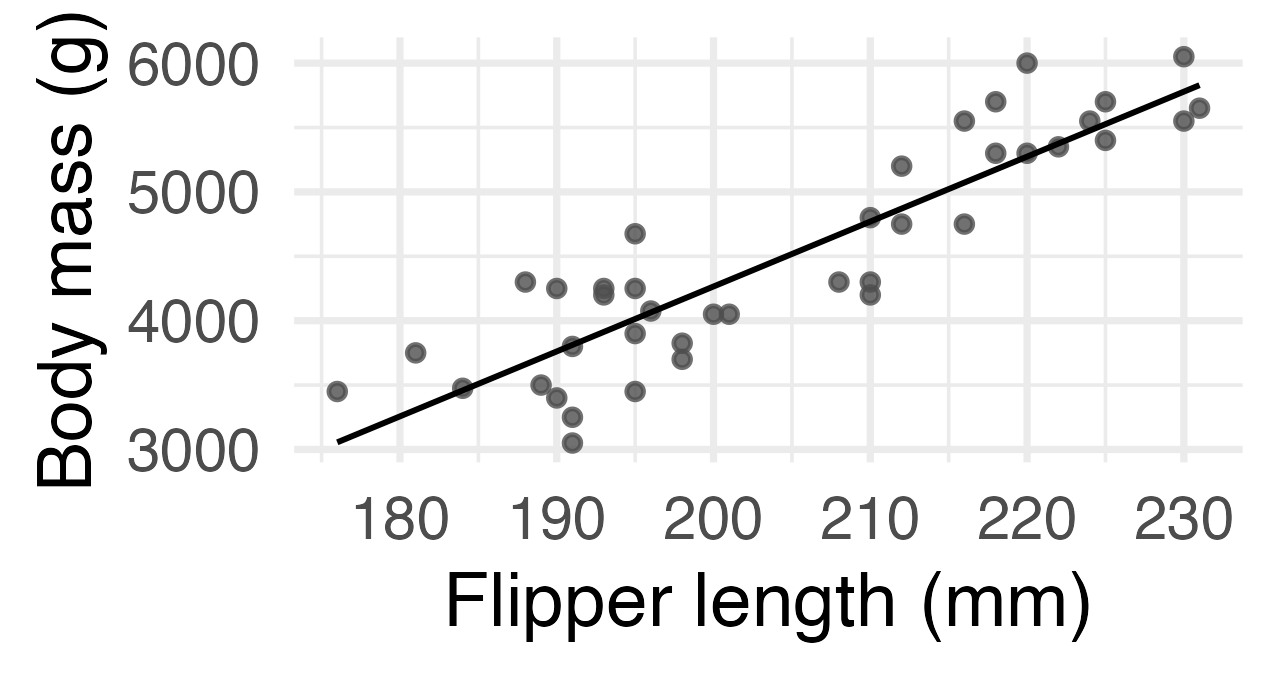
\includegraphics[width=0.46\textwidth]{penguins_scatter.png}
\end{center}

\vspace{-0.3em}
\dq{The fitted slope is $\hat\beta_1 = 50.4$ g/mm, from $40$ penguins rather than all penguins. Could a \emph{flat} truth produce a tilt this steep by chance?}

\end{frame}


\section{Two roads to the null distribution}

%%%%%%%%%%%%%%%%%%%%%%%%%%%%%%%%%%%%%%%%%%%%%%%%%%%%%%%%%%%%%%%%%%%%%%%%
\begin{frame}
\frametitle{Road A: shuffle the pairing}
\examplehead{Palmer penguins}

Under $H_0:\beta_1 = 0$, which mass belongs to which flipper is arbitrary: the pairing is \hl{exchangeable}. Shuffle the masses, refit, record the slope, repeat.

\vspace{-0.2em}
\begin{center}
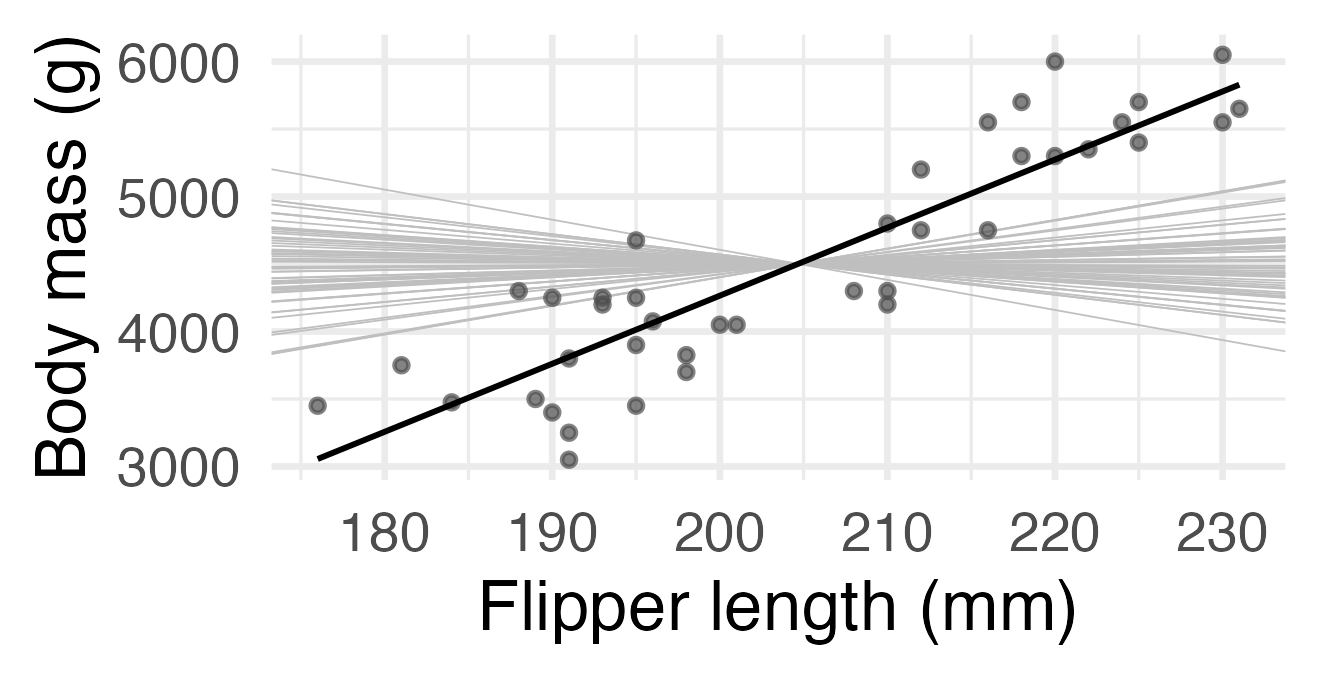
\includegraphics[width=0.52\textwidth]{perm_lines.png}
\end{center}

\vspace{-0.3em}
{\small Each grey line is one shuffle, scattering around \emph{flat}. The real line (black) is far steeper: a small p-value, seen.}

\end{frame}


%%%%%%%%%%%%%%%%%%%%%%%%%%%%%%%%%%%%%%%%%%%%%%%%%%%%%%%%%%%%%%%%%%%%%%%%
\begin{frame}
\frametitle{Road B: the $t$ model}

The $t$ distribution from Lecture 10 returns here, for the slope.

\vspace{0.2em}
\formula{Inference for the slope}{
\[
\mathrm{SE}(\hat\beta_1) = \frac{s_e}{s_x\sqrt{n-1}},
\qquad
T = \frac{\hat\beta_1}{\mathrm{SE}(\hat\beta_1)} \sim t_{n-2}.
\]}

\vspace{0.2em}
{\small
\begin{itemize}\setlength{\itemsep}{1pt}
\item $s_e$ is the spread of the residuals, $s_x$ the spread of $x$. A slope is easier to pin down when the points hug the line and the $x$'s spread wide.
\item Why $t_{n-2}$? Placing a line costs \emph{two} estimates, slope and intercept, one more than a single mean.
\item \hl{The shortcut has conditions}, checked shortly.
\end{itemize}}

\end{frame}


%%%%%%%%%%%%%%%%%%%%%%%%%%%%%%%%%%%%%%%%%%%%%%%%%%%%%%%%%%%%%%%%%%%%%%%%
\begin{frame}[fragile]
\frametitle{Road A in R}
\examplehead{Palmer penguins}

\begin{lstlisting}[language=R, basicstyle=\ttfamily\scriptsize]
t_of <- function(x, y) ...          # slope / SE(slope)

t_obs <- t_of(peng$flipper, peng$mass)     # 12.3

null <- replicate(10000,
  t_of(peng$flipper, sample(peng$mass)))   # shuffle!

mean(abs(null) >= abs(t_obs))              #> 0 (p<0.001)
\end{lstlisting}

\vspace{-0.2em}
{\small We record the scale-free $t = \hat\beta_1/\mathrm{SE}$ from Road B, shuffle, and count how often $|t|$ beats the observed $12.3$. It never does. Taking $|t|$ makes the test \hl{two-sided}: a slope that is too \emph{negative} is evidence against $H_0:\beta_1=0$ just as much as one that is too positive.}

\end{frame}


%%%%%%%%%%%%%%%%%%%%%%%%%%%%%%%%%%%%%%%%%%%%%%%%%%%%%%%%%%%%%%%%%%%%%%%%
\begin{frame}
\frametitle{And the two roads agree}
\examplehead{Palmer penguins}

\vspace{-0.2em}
\begin{center}
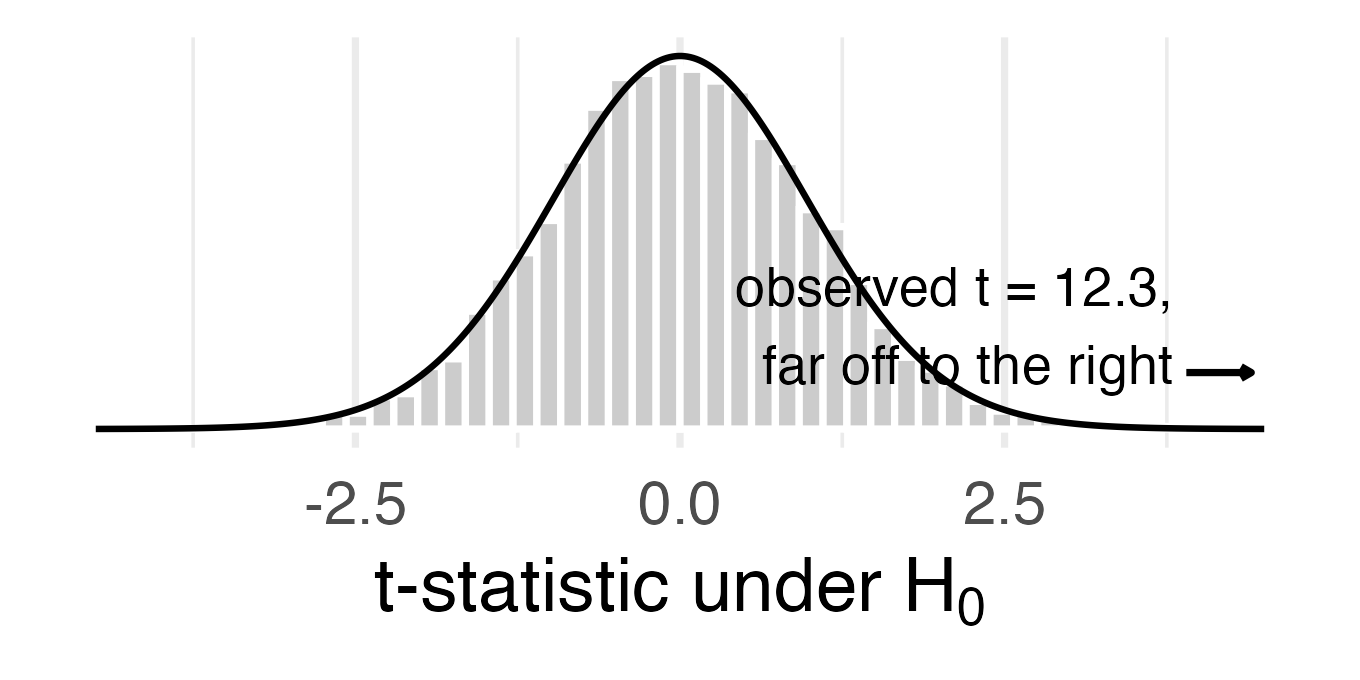
\includegraphics[width=0.60\textwidth]{slope_null_overlay.png}
\end{center}

\vspace{-0.3em}
\keyidea{The shuffled $t$-statistics pile up into exactly the $t_{38}$ curve: mean $0.01$ (theory $0$), SD $1.03$ (theory $1.03$). Both roads give $p < 0.001$, and the observed $t = 12.3$ is far beyond either.}

\end{frame}


\section{A confidence interval, two ways}

%%%%%%%%%%%%%%%%%%%%%%%%%%%%%%%%%%%%%%%%%%%%%%%%%%%%%%%%%%%%%%%%%%%%%%%%
\begin{frame}
\frametitle{Plausible slopes: bootstrap the pairs}
\examplehead{Palmer penguins}

For a \emph{range} of plausible slopes, resample whole $(x, y)$ \hl{pairs} with replacement, so the $x$--$y$ link survives. Refit, collect the slope.

\vspace{-0.1em}
\begin{center}
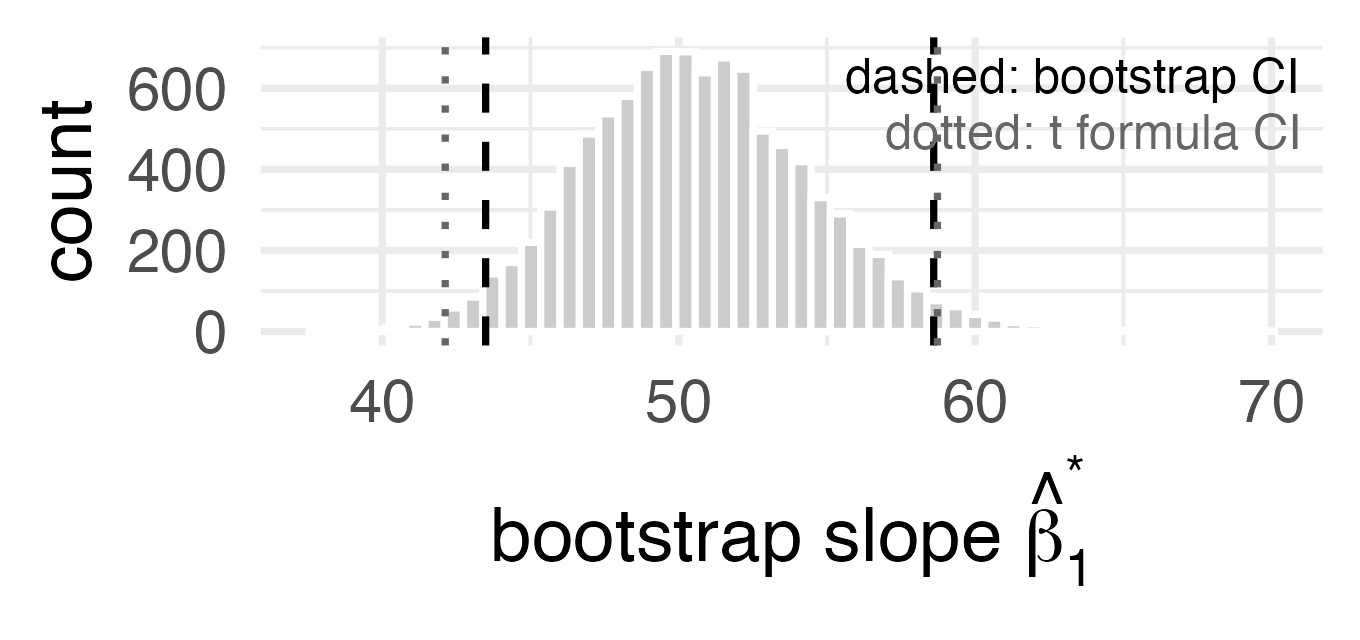
\includegraphics[width=0.6\textwidth]{slope_boot_ci.png}
\end{center}

\vspace{-0.3em}
{\small Bootstrap CI $[43.5, 58.6]$ versus the formula's $\hat\beta_1 \pm t^\ast\,\mathrm{SE} = [42.1, 58.7]$, with $t^\ast$ the critical value from $t_{n-2}$. The same interval, two ways.}

\end{frame}


\section{Checking model conditions}

%%%%%%%%%%%%%%%%%%%%%%%%%%%%%%%%%%%%%%%%%%%%%%%%%%%%%%%%%%%%%%%%%%%%%%%%
\begin{frame}
\frametitle{The formula's conditions: LINE}

The $t_{n-2}$ shortcut is trustworthy only under four conditions, \hl{LINE}:

\vspace{0.1em}
\begin{enumerate}
\item \textbf{L}inearity: the trend really is a straight line.
\item \textbf{I}ndependence: observations do not influence one another.
\item \textbf{N}ormality: the residuals are roughly normal.
\item \textbf{E}qual variance: residual spread is constant across $x$.
\end{enumerate}

\vspace{0.2em}
\caution{%
\begin{itemize}\setlength{\itemsep}{1pt}
\item Check on the \emph{residuals}: residuals-vs-fitted for L and E, Q--Q for N, the design for I.
\item Both simulations need I too. Only the bootstrap adapts to unequal variance.
\end{itemize}}

\end{frame}


%%%%%%%%%%%%%%%%%%%%%%%%%%%%%%%%%%%%%%%%%%%%%%%%%%%%%%%%%%%%%%%%%%%%%%%%
\begin{frame}
\frametitle{Checking LINE on the penguins}
\examplehead{Palmer penguins}

\vspace{-0.2em}
\twocol{0.5}{0.5}
{
\begin{center}
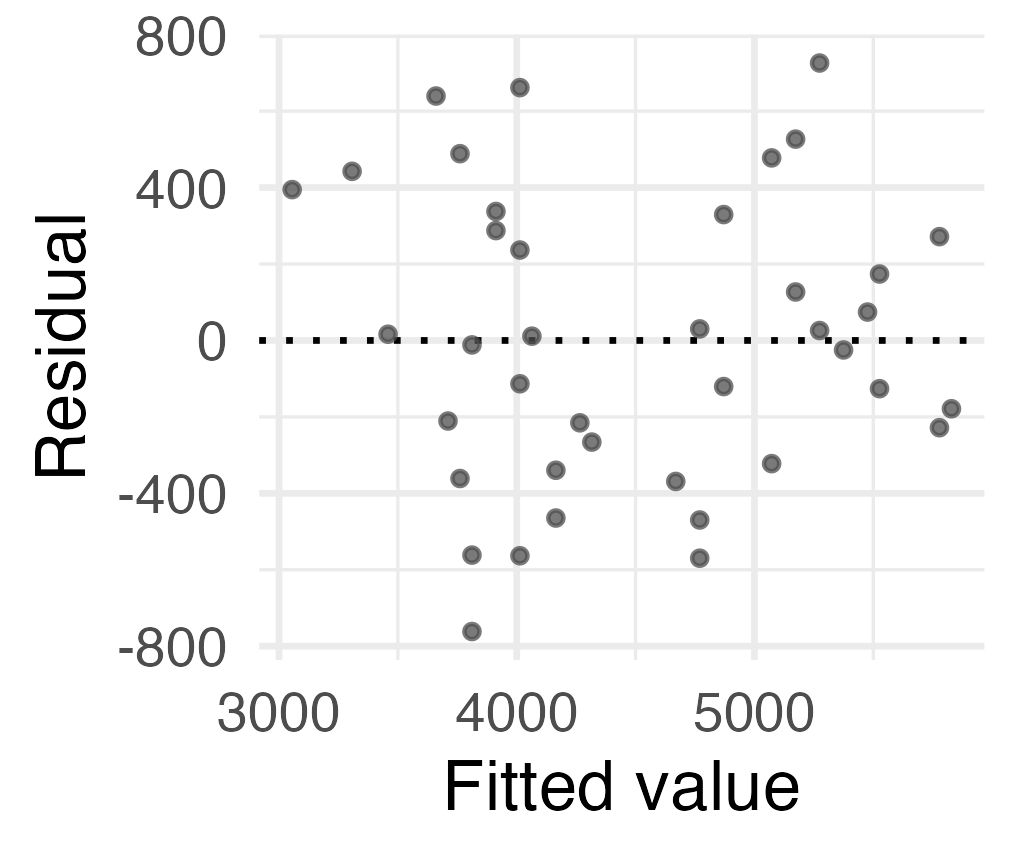
\includegraphics[width=0.94\textwidth]{resid_fitted.png}
\end{center}
}
{
\begin{center}
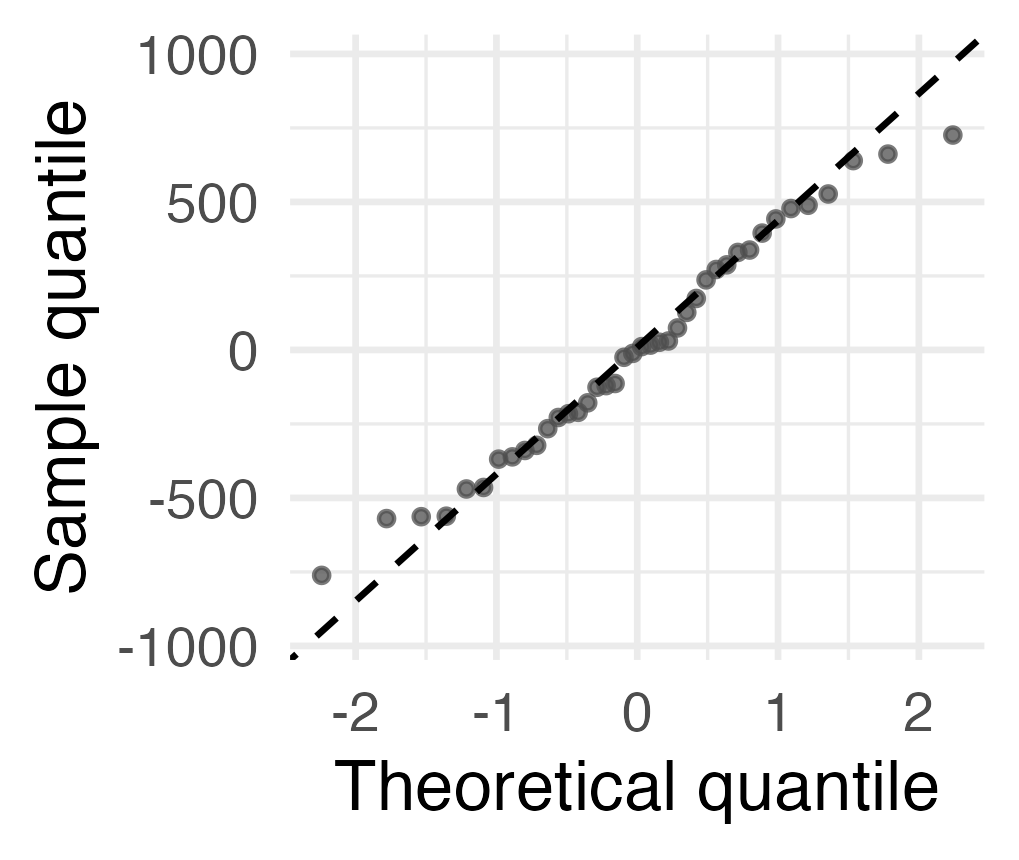
\includegraphics[width=0.94\textwidth]{qq.png}
\end{center}
}

\vspace{-0.2em}
{\small \textbf{Left:} residuals flat around zero with even spread, so L and E look fine. \textbf{Right:} points hug the line, so N is reasonable. The \hl{same diagnostics as ANOVA} (Lecture 12): both are the one linear model.}

\end{frame}


%%%%%%%%%%%%%%%%%%%%%%%%%%%%%%%%%%%%%%%%%%%%%%%%%%%%%%%%%%%%%%%%%%%%%%%%
\begin{frame}
\frametitle{What a broken condition looks like}

\vspace{-0.2em}
\begin{center}
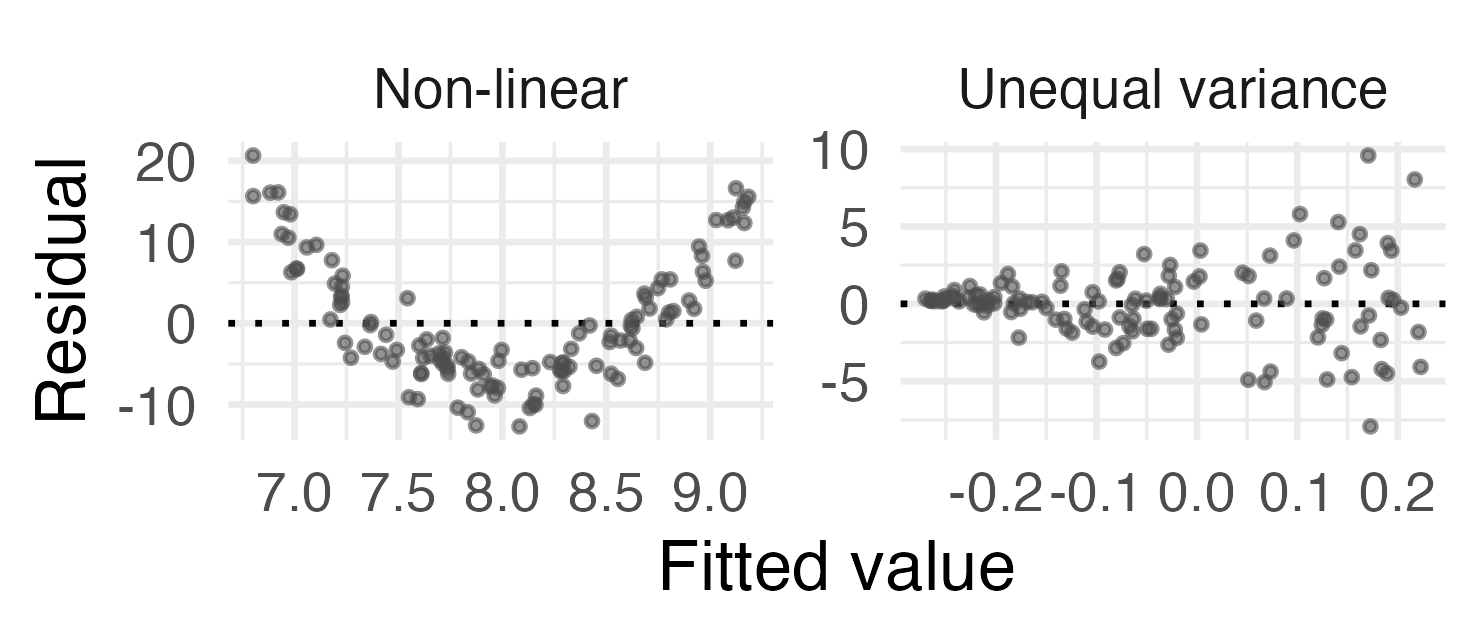
\includegraphics[width=0.85\textwidth]{violations_grid.png}
\end{center}

\vspace{-0.3em}
{\small A \emph{curve} in the residuals means the relationship is not linear. A \emph{funnel} means the variance is not constant. Either way the formula is not to be trusted.}

\end{frame}


%%%%%%%%%%%%%%%%%%%%%%%%%%%%%%%%%%%%%%%%%%%%%%%%%%%%%%%%%%%%%%%%%%%%%%%%
\begin{frame}
\frametitle{When the two roads \emph{disagree}}
\examplehead{Loans}

Loan amount vs.\ annual income, $400$ loans.

\vspace{-0.2em}
\begin{center}
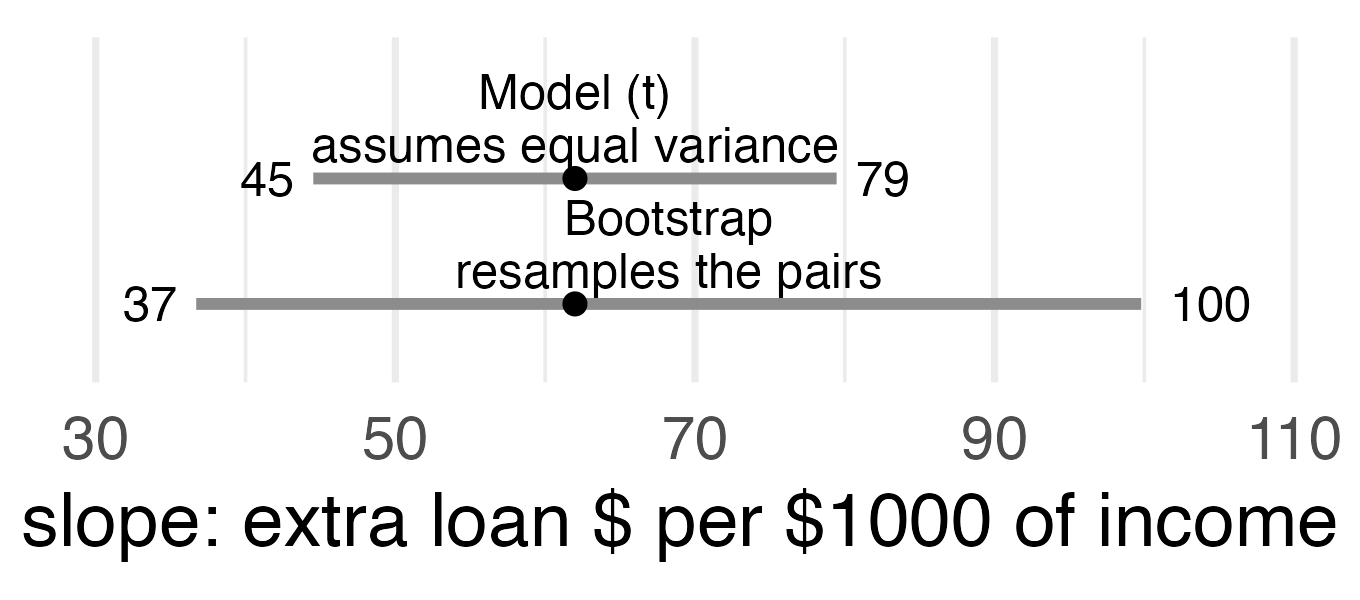
\includegraphics[width=0.52\textwidth]{loans_ci.png}
\end{center}

\vspace{-0.3em}
\caution{Bigger incomes bring far more variable loans, so equal variance fails. The $t$ CI is too narrow. The bootstrap tracks the changing spread.}

\end{frame}


%%%%%%%%%%%%%%%%%%%%%%%%%%%%%%%%%%%%%%%%%%%%%%%%%%%%%%%%%%%%%%%%%%%%%%%%
\begin{frame}
\frametitle{A remedy: transform, then re-check}
\examplehead{Loans}

\vspace{-0.3em}
\begin{center}
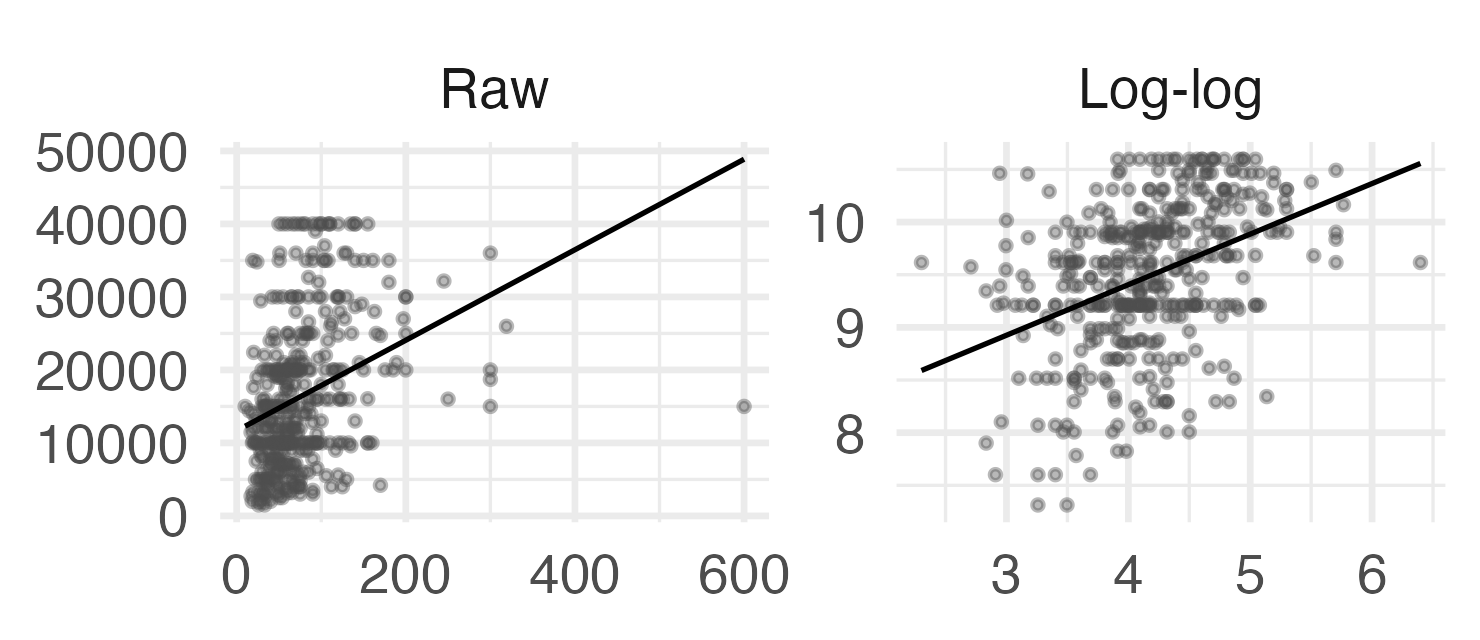
\includegraphics[width=0.66\textwidth]{loans_resid_fix.png}
\end{center}

\vspace{-0.3em}
\keyidea{Modeling $\log(\texttt{loan})$ on $\log(\texttt{income})$ steadies the spread (funnel indicator $0.25 \to -0.12$), so LINE holds and the two roads re-agree. The slope is now an \hl{elasticity}: $1\%$ more income predicts about $0.48\%$ more loan.}

\end{frame}


\section{Reading the output; the intercept}

%%%%%%%%%%%%%%%%%%%%%%%%%%%%%%%%%%%%%%%%%%%%%%%%%%%%%%%%%%%%%%%%%%%%%%%%
\begin{frame}[fragile]
\frametitle{Reading it straight off \texttt{lm()}}
\examplehead{Palmer penguins}

\begin{lstlisting}[language=R, basicstyle=\ttfamily\scriptsize]
lm(body_mass_g ~ flipper_length_mm, data = peng) |>
  tidy(conf.int = TRUE)

  term               estimate  std.error  statistic  p.value
  (Intercept)          -5820        842      -6.92    <0.001
  flipper_length_mm       50.4        4.1     12.3     <0.001
                     conf.low  conf.high
                       -7523      -4116
                        42.1       58.7
\end{lstlisting}

\vspace{-0.2em}
{\small The \texttt{flipper} row \emph{is} Road B: estimate $50.4$, $\mathrm{SE}$ $4.1$, $t = 12.3$, CI $[42.1, 58.7]$. One extra mm of flipper predicts about $50$ g more mass.}

\end{frame}


%%%%%%%%%%%%%%%%%%%%%%%%%%%%%%%%%%%%%%%%%%%%%%%%%%%%%%%%%%%%%%%%%%%%%%%%
\begin{frame}
\frametitle{The intercept: often a nonsense point}
\examplehead{Palmer penguins}

$\hat\beta_0 = -5820$ g is the predicted mass at flipper length $= 0$ mm.

\vspace{0.3em}
{\small A penguin with no flipper does not weigh $-5820$ g. The intercept sits far outside the data (flippers run $172$--$231$ mm), so it \emph{anchors} the line but has no meaning on its own.}

\pause
\vspace{0.3em}
\keyidea{Interpret and test the intercept only when $x = 0$ is near the data. Its confidence interval is built exactly like the slope's: $\hat\beta_0 \pm t^\ast\,\mathrm{SE}(\hat\beta_0)$.}

\end{frame}


%%%%%%%%%%%%%%%%%%%%%%%%%%%%%%%%%%%%%%%%%%%%%%%%%%%%%%%%%%%%%%%%%%%%%%%%
\begin{frame}
\frametitle{Testing a slope against a value other than zero}

Sometimes the question is not ``is the slope zero?'' but ``is it some particular $c$?''

\vspace{0.2em}
\formula{A general slope test}{
\[
t = \frac{\hat\beta_1 - c}{\mathrm{SE}(\hat\beta_1)} \sim t_{n-2}
\qquad \text{under } H_0:\beta_1 = c.
\]}

\vspace{0.2em}
{\small Setting $c = 0$ recovers the usual test. And note the \hl{duality with the CI}: a value $c$ lies inside the $95\%$ CI \emph{exactly when} the test does not reject $\beta_1 = c$ at the $5\%$ level. Here $40$ sits just below $[42.1, 58.7]$, so we would (barely) reject $\beta_1 = 40$.}

\end{frame}


\section{Wrap-up}

%%%%%%%%%%%%%%%%%%%%%%%%%%%%%%%%%%%%%%%%%%%%%%%%%%%%%%%%%%%%%%%%%%%%%%%%
\begin{frame}
\frametitle{The same two roads, now in regression}

{\scriptsize
\begin{center}
\setlength{\tabcolsep}{2.5pt}
\begin{tabular}{lll}
\toprule
\textbf{The statistic} & \textbf{By simulation} & \textbf{By formula} \\
\midrule
a proportion & simulate $H_0$ (Lec 8) & binomial, exact; $z$ (Lec 10) \\
a mean or a difference & bootstrap (Lec 9), permute (Lec 8) & the CLT: $z$, $t$ (Lec 10) \\
a whole table, $X^2$ & permute one column (Lec 11) & $\chi^2_{df}$ (Lec 11) \\
several group means, $F$ & permute the labels (Lec 12) & $F_{df_1,df_2}$ (Lec 12) \\
\hl{a regression slope, $\hat\beta_1$} & \hl{shuffle / bootstrap pairs (today)} & \hl{$t_{n-2}$ (today)} \\
\bottomrule
\end{tabular}
\end{center}}

\vspace{0.3em}
\emph{State $H_0$, build a statistic, get its null two ways, then see how extreme the data are}, now for the slope of a line.

\end{frame}


%%%%%%%%%%%%%%%%%%%%%%%%%%%%%%%%%%%%%%%%%%%%%%%%%%%%%%%%%%%%%%%%%%%%%%%%
\begin{frame}
\frametitle{Summary}

\begin{itemize}
\item A fitted slope is an \emph{estimate}: ask whether its tilt is real, and which values are plausible.
\item Test $H_0:\beta_1 = 0$ two roads, \hl{shuffle the pairing} or $T = \hat\beta_1/\mathrm{SE} \sim t_{n-2}$. On the penguins both gave $p < 0.001$.
\item Interval two roads, \hl{bootstrap the pairs} or $\hat\beta_1 \pm t^\ast\,\mathrm{SE}$. Both gave about $[42, 59]$ g/mm.
\item The formula needs \hl{LINE}; read it off residual and Q--Q plots. If it fails, transform or trust the simulation.
\item Pull $\hat\beta_1$, its SE, $t$, and CI straight from \texttt{lm()}/\texttt{tidy()}, and check whether the intercept is even meaningful.
\end{itemize}

\end{frame}


%%%%%%%%%%%%%%%%%%%%%%%%%%%%%%%%%%%%%%%%%%%%%%%%%%%%%%%%%%%%%%%%%%%%%%%%
\begin{frame}
\frametitle{Coming up next}

\hl{Next, multiple regression:} more than one predictor at once. Today's slope test becomes one \emph{row} of the \texttt{lm()} table, with $df$ going $n-2 \to n-p-1$ and each slope read ``holding the others fixed'' (IMS Ch.\ 25).

\vspace{0.4em}
{\small The $t$ statistic, the CI, the LINE conditions and the residual plots all carry over unchanged.}

\end{frame}


%%%%%%%%%%%%%%%%%%%%%%%%%%%%%%%%%%%%%%%%%%%%%%%%%%%%%%%%%%%%%%%%%%%%%%%%
% Activity
%%%%%%%%%%%%%%%%%%%%%%%%%%%%%%%%%%%%%%%%%%%%%%%%%%%%%%%%%%%%%%%%%%%%%%%%

\begin{frame}
\frametitle{Activity: do heavier kangaroo rats have longer feet?}

\activity{The Portal kangaroo rats from Lectures 9--10: the same $347$ animals, a new question. Fit \texttt{weight \textasciitilde{} hindfoot\_length}, then
\begin{itemize}\setlength{\itemsep}{1pt}
\item test the slope both ways: shuffle vs.\ the $t$ formula;
\item bound it both ways: bootstrap vs.\ $\hat\beta_1 \pm t^\ast\,\mathrm{SE}$;
\item check LINE on the residuals. Do the two roads agree?
\end{itemize}}

\vspace{0.3em}
{\small
\begin{itemize}
\item Work in \emph{pairs} (analyst + guide); one worksheet per pair.
\item We pause for check-ins. \hl{Be ready to share}.
\item Data and starter code are on Blackboard.
\end{itemize}}

\end{frame}



%%%%%%%%%%%%%%%%%%%%%%%%%%%%%%%%%%%%
% End document
%%%%%%%%%%%%%%%%%%%%%%%%%%%%%%%%%%%%

\end{document}
